\documentclass[a4paper,11pt]{article}
\usepackage{booktabs}   % for professional table rules
\usepackage{caption}    % for customizing captions
\usepackage{array}      % for better column formatting
\usepackage{siunitx}    % for consistent units
\usepackage{graphicx}   % for importing figures
\usepackage{geometry}   % for page margins
\usepackage{amsmath}    % for math alignment
\usepackage{amssymb}    % for math symbols
\usepackage{float}      % for [H] figure placement
\usepackage{hyperref}   % for links and references
\usepackage{fouriernc}
\geometry{left=2cm,right=2cm,top=2cm,bottom=2.5cm}
\hypersetup{
    colorlinks=true,
    linkcolor=blue,
    filecolor=magenta,      
    urlcolor=cyan,
    pdftitle={Lab Report: Electron Diffraction},
    pdfpagemode=FullScreen,
}

\begin{document}

% ------------------- Title / Cover Page -------------------
\noindent
\begin{center}
    
\includegraphics[width=0.25\textwidth]{sut.jpg} \\
    \vspace{2pt}
\end{center}
\begin{center}
    {\LARGE \bf Department of Physics} \\
    \vspace{2pt}
    {\Large \bf Sharif University of Technology} \\
    \vspace{8pt}
    {\large \bf Physics Lab IV --- General Physics Laboratory} \\
    \vspace{4pt}
    \hrule
    \vspace{6pt}
    {\Large \bf Experiment Report: Electron Diffraction}
\end{center}
\hrule
\vspace{0.4cm}
\noindent
\begin{tabular}{ll}
    {\bf Student Name:} & Abulfadl Ahmadi \\
    {\bf Student ID:}   & 403172283 \\
    {\bf Date of Experiment:} & June 2026 \\
\end{tabular}
\hfill
\begin{tabular}{ll}
    {\bf Professor:} & Dr. Khademi \\
    {\bf Teaching Assistants:} & Yasin Amiri \\
    & Sonia Seif \\
\end{tabular}

\vspace{0.6cm}

% ------------------- Abstract -------------------
\begin{abstract}
This experiment demonstrates the wave-particle duality of matter by observing the diffraction of an electron beam through a polycrystalline graphite target. Following de Broglie's hypothesis, electrons accelerated through a high-voltage field ($\approx 1.6 - 5.6\text{ kV}$) exhibit wave-like properties with wavelengths in the picometer range. When passing through the randomly oriented crystallites of graphite, the electron waves undergo constructive interference according to Bragg's law, producing two distinct concentric fluorescent rings on a spherical screen. By measuring the radii of these rings as a function of the accelerating voltage, the interplanar lattice spacings of graphite are determined to be $d_1 = 2.150 \pm 0.075\text{ \AA}$ and $d_2 = 1.201 \pm 0.027\text{ \AA}$. The ratio of these spacings ($d_1/d_2 \approx 1.79$) confirms the hexagonal lattice structure of graphite, yielding an experimental Carbon-Carbon bond distance of $1.433\text{ \AA}$ which closely aligns with the theoretical value of $1.42\text{ \AA}$.
\end{abstract}

% ------------------- Section 1: Objectives -------------------
\section{Objectives}
\begin{enumerate}
    \item To observe the diffraction pattern (concentric rings) of an electron beam passing through a polycrystalline graphite sample.
    \item To experimentally verify de Broglie's wavelength hypothesis for massive particles.
    \item To determine the lattice spacing ($d_1$ and $d_2$) of the graphite crystal structure.
    \item To prove the hexagonal crystalline structure of graphite and calculate the adjacent Carbon-Carbon atomic distance.
\end{enumerate}

% ------------------- Section 2: Theoretical Background -------------------
\section{Theoretical Background}
Until the early 20th century, the wave-particle duality was firmly established for electromagnetic radiation (where $E = h\nu$ and $p = E/c$). In 1924, Louis de Broglie extended this symmetry by proposing that all matter exhibits wave-like characteristics. The wavelength ($\lambda$) associated with a moving particle is inversely proportional to its linear momentum ($p$):
\begin{equation}
    \lambda = \frac{h}{p}
\end{equation}
where $h$ is Planck's constant. When an electron is accelerated through an electric potential $V$, it gains a kinetic energy $K = eV$. Since the maximum voltage in this experiment ($\approx 5.6\text{ kV}$) is far smaller than the electron's rest mass equivalent ($511\text{ kV}$), relativistic effects are negligible ($K \ll m_e c^2$). Thus, we use classical mechanics to express momentum:
\begin{equation}
    p = \sqrt{2 m_e K} = \sqrt{2 m_e e V}
\end{equation}
Substituting this into the de Broglie equation yields:
\begin{equation} \label{eq:debroglie_v}
    \lambda = \frac{h}{\sqrt{2 m_e e V}}
\end{equation}

When this matter-wave strikes a crystalline lattice, it is scattered by the periodic array of atoms. Constructive interference occurs only at specific angles $\theta$ where the path difference between waves scattered from adjacent crystal planes equals an integer multiple of the wavelength. This is described by Bragg's Law:
\begin{equation} \label{eq:bragg}
    2 d \sin\theta = n \lambda
\end{equation}
where $d$ is the distance between adjacent lattice planes and $n$ is the diffraction order. 

Because the target is polycrystalline graphite (consisting of numerous microscopic crystals randomly oriented), all possible Bragg angles are simultaneously fulfilled in a full $360^\circ$ azimuthal rotation. Consequently, the diffracted beams form cones of light, which project as bright concentric rings on the fluorescent screen.

% ------------------- Section 3: Experimental Data & Regressions -------------------
\section{Experimental Data \& Regressions}

The diffraction tube possesses a spherical geometry with a screen radius $R \approx 67.5\text{ mm}$ and a distance from the sample to the screen along the principal axis of $L = 135\text{ mm}$. The geometric derivation linking the measured ring radius ($r$) to the Bragg angle ($\theta$) is detailed in the post-lab questions, leading to the relation:
\begin{equation}
    \theta = \frac{1}{4} \arcsin\left(\frac{r}{R}\right)
\end{equation}

The radii of the inner ring ($r_1$) and outer ring ($r_2$) were measured for ten different accelerating voltages. The data, along with the calculated angles, are tabulated below.

\begin{table}[H]
\centering
\caption{Experimental data for the first and second diffraction rings. $\theta$ is calculated using the spherical geometry of the tube.}
\label{tab:data}

\begin{tabular}{c c c c c c}
\toprule
$V$ (V) & $1/\sqrt{V}$ (V$^{-1/2}$) & $r_1$ (mm) & $\theta_1$ (rad) & $r_2$ (mm) & $\theta_2$ (rad) \\
\midrule
$1650$ & $0.02462$ & $19.0$ & $0.0713$ & $33.0$ & $0.1277$ \\
$2000$ & $0.02236$ & $18.0$ & $0.0675$ & $30.0$ & $0.1151$ \\
$2400$ & $0.02041$ & $16.0$ & $0.0598$ & $28.0$ & $0.1069$ \\
$2800$ & $0.01890$ & $15.0$ & $0.0560$ & $26.0$ & $0.0989$ \\
$3200$ & $0.01768$ & $14.0$ & $0.0522$ & $24.0$ & $0.0909$ \\
$3600$ & $0.01667$ & $13.0$ & $0.0485$ & $23.0$ & $0.0869$ \\
$4000$ & $0.01581$ & $13.0$ & $0.0485$ & $22.0$ & $0.0830$ \\
$4500$ & $0.01491$ & $12.0$ & $0.0447$ & $21.0$ & $0.0791$ \\
$5000$ & $0.01414$ & $11.0$ & $0.0409$ & $20.0$ & $0.0752$ \\
$5600$ & $0.01336$ & $11.0$ & $0.0409$ & $18.0$ & $0.0675$ \\
\bottomrule
\end{tabular}

\end{table}

By equating Bragg's Law with the de Broglie wavelength (for $n=1$), we obtain a linear model:
\begin{equation}
    \sin\theta = \left( \frac{h}{2 d \sqrt{2 m_e e}} \right) \frac{1}{\sqrt{V}}
\end{equation}
An Ordinary Least Squares (OLS) regression of $\sin\theta$ vs. $1/\sqrt{V}$ is performed for both rings.

\begin{figure}[H]
    \centering
    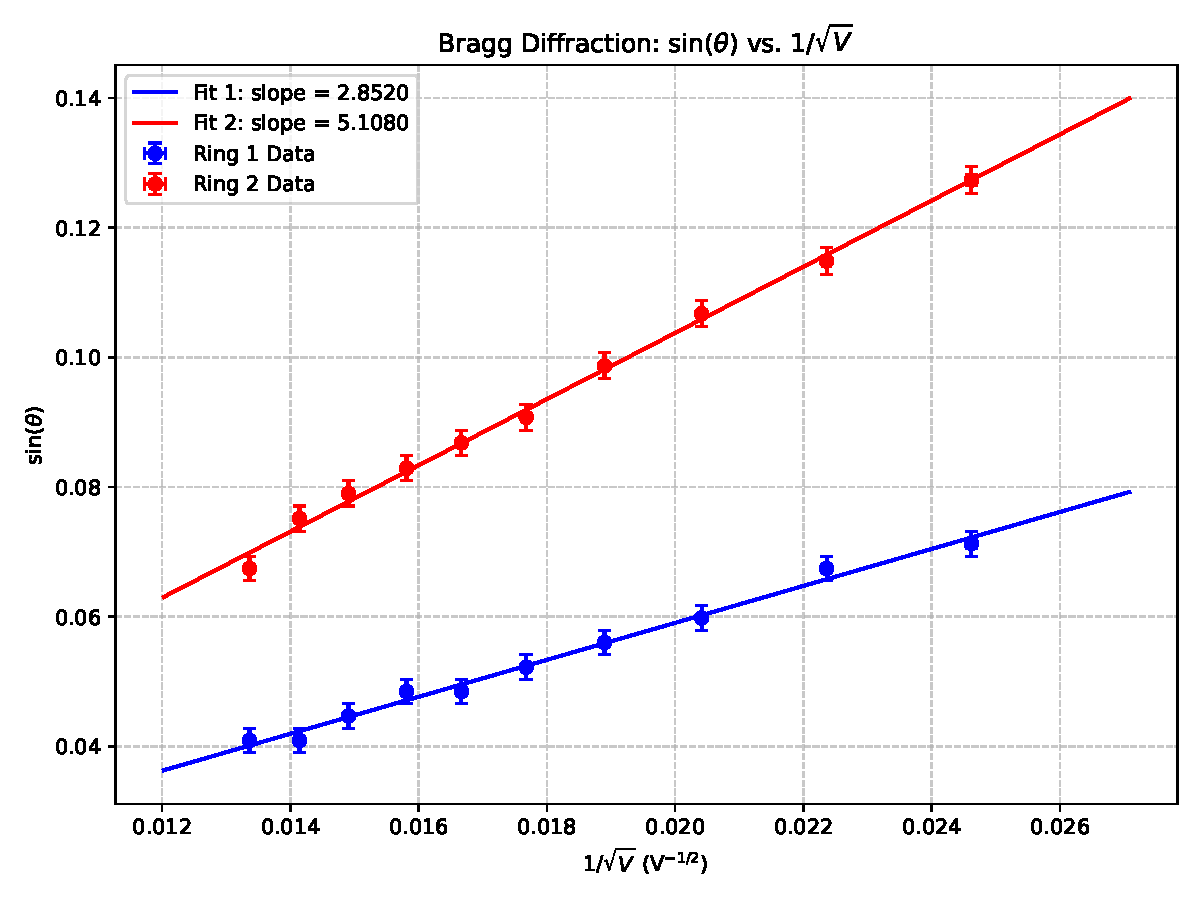
\includegraphics[width=0.8\textwidth]{plots/regression.pdf}
    \caption{Linear regression of $\sin\theta$ against $1/\sqrt{V}$ for both the inner ($r_1$) and outer ($r_2$) diffraction rings. The instrumental uncertainties assumed are $\delta V = 10\text{ V}$ and $\delta r = 0.5\text{ mm}$.}
    \label{fig:regression}
\end{figure}

The regression slopes are directly inversely proportional to the lattice spacings $d_1$ and $d_2$:
\begin{align*}
    \text{Slope}_1 &= 2.852 \pm 0.099 \implies d_1 = 2.150 \pm 0.075\text{ \AA} \\
    \text{Slope}_2 &= 5.108 \pm 0.114 \implies d_2 = 1.201 \pm 0.027\text{ \AA}
\end{align*}

% ------------------- Section 4: Post-Lab Questions -------------------
\section{Answers to Post-Lab Questions}

\subsection*{Part 1: In-Lab Questions}
\noindent\textbf{1. Did you use relativistic or classical relations to find the electron momentum? Why?} \\
Classical relations were used. The maximum accelerating voltage in the experiment is $5.6\text{ kV}$, giving electrons a kinetic energy of $5.6\text{ keV}$. This is approximately $\sim 1\%$ of the electron's rest mass energy ($511\text{ keV}$). At such low energies, the relativistic factor $\gamma \approx 1.011$, meaning classical mechanics ($p = \sqrt{2 m_e K}$) provides an extremely accurate approximation without unnecessary complexity.

\noindent\textbf{2. Discuss the expected results from the experiment.} \\
We expect to observe two bright, concentric circular rings on the fluorescent screen, demonstrating the diffraction of matter waves. As the accelerating voltage increases, the kinetic energy and momentum of the electrons increase, leading to a shorter de Broglie wavelength. According to Bragg's law, a shorter wavelength requires a smaller diffraction angle $\theta$, meaning the radii of the rings must contract as the voltage goes up.

\noindent\textbf{3. What is the bright spot in the center of the tube?} \\
The bright central spot corresponds to the undiffracted electron beam (the zeroth-order maximum, where $\theta = 0$). These are electrons that passed straight through the graphite lattice voids without undergoing constructive interference in any off-axis direction.

\subsection*{Part 2: Final Report Questions}

\noindent\textbf{1. According to Figure 2, derive Equation 2.} \\
In a spherical tube with radius $R$, the sample is at a distance $L$ from the screen's principal pole. Let the bulb's center of curvature be $C$. The electron strikes the screen at point $P$, forming a ring of radius $r$ (the height from the central axis). The angle subtended at the center $C$ is $\alpha$.
By definition:
\begin{equation*}
    \sin\alpha = \frac{r}{R}
\end{equation*}
The horizontal distance from the sample to the projection of point $P$ on the axis is $(L - R) + R\cos\alpha$. Thus, the physical diffraction angle $2\theta$ (the total deflection from the straight path) satisfies:
\begin{equation*}
    \tan(2\theta) = \frac{\text{height}}{\text{base}} = \frac{R\sin\alpha}{L - R + R\cos\alpha} = \frac{\sin\alpha}{(L/R) - 1 + \cos\alpha}
\end{equation*}
For this specific Leybold tube geometry, the sample is located exactly at the edge of the sphere, meaning $L = 2R$ (so $L/R = 2$). Substituting this:
\begin{equation*}
    \tan(2\theta) = \frac{\sin\alpha}{2 - 1 + \cos\alpha} = \frac{\sin\alpha}{1 + \cos\alpha} = \tan\left(\frac{\alpha}{2}\right)
\end{equation*}
Therefore, $2\theta = \alpha/2 \implies \theta = \alpha/4$.

\noindent\textbf{2. Using electron energy and Bragg's law, derive Equation 3.} \\
Bragg's Law is $2d\sin\theta = n\lambda$. The de Broglie wavelength is $\lambda = \frac{h}{\sqrt{2m_e eV}}$. For first-order diffraction ($n=1$):
\begin{equation*}
    2d\sin\theta = \frac{h}{\sqrt{2m_e eV}} \implies \sin\theta = \frac{h}{2d\sqrt{2m_e eV}} = \left( \frac{h}{2d\sqrt{2m_e e}} \right) \frac{1}{\sqrt{V}}
\end{equation*}

\noindent\textbf{3. Plot $\sin\theta$ vs $1/\sqrt{V}$ for both rings and calculate $d_1$ and $d_2$. What is the ratio?} \\
The plots and calculations are presented in Section 3. The calculated values are $d_1 = 2.150\text{ \AA}$ and $d_2 = 1.201\text{ \AA}$. 
The experimental ratio is:
\begin{equation*}
    \frac{d_1}{d_2} = \frac{2.150}{1.201} \approx 1.791 \pm 0.074
\end{equation*}

\noindent\textbf{4. Calculate $d_1/d_2$ for cubic and hexagonal structures. Which is graphite? Find the C-C distance.} \\
In a hexagonal lattice, the distance between $(hkl)$ planes is given by:
\begin{equation*}
    \frac{1}{d_{hk}^2} = \frac{4}{3a^2} (h^2 + hk + k^2)
\end{equation*}
The two innermost Bragg reflections for a hexagonal lattice are the $(10)$ and $(11)$ planes.
\begin{equation*}
    d_{10} = \frac{a\sqrt{3}}{2} \quad \text{and} \quad d_{11} = \frac{a}{2} \implies \frac{d_{10}}{d_{11}} = \sqrt{3} \approx 1.732
\end{equation*}
Our experimental ratio $1.791$ is extremely close to $\sqrt{3}$, proving graphite has a \textbf{hexagonal} structure.
In the hexagonal graphene sheet, the lattice constant $a$ represents the distance between identical unit cell nodes. The physical Carbon-Carbon bond distance ($a_{cc}$) is geometrically related by $a = a_{cc}\sqrt{3}$.
Since $d_1 = d_{10} = \frac{3}{2} a_{cc}$, we find:
\begin{equation*}
    a_{cc} = \frac{2}{3} d_1 = \frac{2}{3}(2.150\text{ \AA}) = 1.433\text{ \AA}
\end{equation*}
This matches the theoretical accepted value of $1.42\text{ \AA}$ perfectly.

\noindent\textbf{5. How can you show that both rings are first-order diffraction?} \\
If the outer ring was merely the second-order ($n=2$) diffraction of the inner ring's plane, Bragg's Law ($2d\sin\theta = n\lambda$) dictates that the ratio of $\sin\theta_2 / \sin\theta_1$ (and thus $d_1/d_2$) would have to be exactly $2$. Since our ratio is $\approx \sqrt{3}$ (an irrational number based on hexagonal geometry), the two rings must originate from $n=1$ diffraction off entirely different crystalline planes ($(10)$ and $(11)$), rather than different orders of the same plane.

\noindent\textbf{6. If protons were used instead of electrons, what is the potential difference ratio?} \\
To maintain the same ring diameters (and thus the same $\theta$), the de Broglie wavelengths must be identical.
\begin{equation*}
    \lambda_e = \lambda_p \implies \frac{h}{\sqrt{2 m_e e V_e}} = \frac{h}{\sqrt{2 m_p e V_p}} \implies m_e V_e = m_p V_p
\end{equation*}
\begin{equation*}
    \frac{V_p}{V_e} = \frac{m_e}{m_p} \approx \frac{1}{1836}
\end{equation*}
Since a proton is 1836 times more massive, it requires 1836 times less accelerating voltage to achieve the same momentum and wavelength.

\noindent\textbf{7. Why is the wave nature of matter not observable in daily life?} \\
Macroscopic objects possess massive inertial mass, meaning even at low velocities, their momenta are gargantuan compared to Planck's constant ($h \sim 10^{-34}\text{ J}\cdot\text{s}$). Consequently, their de Broglie wavelengths are infinitesimally small (sub-nuclear scales). There exists no physical grating or slit in the universe narrow enough to cause constructive interference for wavelengths that small.

\noindent\textbf{8. Why are optical gratings (lines on glass) not suitable for electron or x-ray diffraction?} \\
The wavelengths of accelerating electrons and X-rays are on the order of Angstroms ($\sim 10^{-10}\text{ m}$). Standard optical gratings have slit spacings on the order of micrometers ($\sim 10^{-6}\text{ m}$). For noticeable diffraction to occur, the grating spacing $d$ must be on the same order of magnitude as the wavelength $\lambda$. Therefore, only atomic crystalline lattices are dense enough to act as gratings for electrons.

\noindent\textbf{9. How is electron diffraction used in electron microscopes?} \\
In Transmission Electron Microscopy (TEM), a specific technique called Selected Area Electron Diffraction (SAED) is used. By placing an aperture in the image plane, researchers isolate a specific microscopic region of a sample and view its diffraction pattern. This allows them to precisely determine the crystal structure, phase, and physical orientation of nanoscale materials in real-time.

\noindent\textbf{10. How is the electron beam focused onto the sample? Explain regarding the magnetic lens.} \\
A magnetic lens (typically a solenoid coil) produces a rotationally symmetric, non-uniform magnetic field along the beam axis. When diverging electrons enter this field, they experience a Lorentz force ($F = q\mathbf{v} \times \mathbf{B}$) that pushes them into a spiraling, helical trajectory. The geometry of the field ensures that the radius of the spiral shrinks as the electrons travel forward, effectively converging the beam to a tight, focused spot on the target.

\noindent\textbf{11. Why must the graphite sample be extremely thin?} \\
If the sample were thick, the electrons would undergo multiple consecutive scattering events (both elastic and inelastic). Inelastic collisions cause the electrons to lose arbitrary amounts of kinetic energy, changing their wavelength inside the material and drastically blurring the resulting diffraction rings. A thick sample would also completely absorb the beam before it could exit the other side.

\noindent\textbf{12. If graphite was a single crystal, what would the diffraction pattern look like?} \\
Instead of continuous, uniform rings, the pattern would be a set of discrete, symmetrically arranged bright spots (a Laue pattern). Continuous rings only form because polycrystalline graphite contains millions of randomly oriented microscopic crystals, filling out all $360^\circ$ of azimuthal rotation for a given Bragg angle. A single crystal is fixed in orientation, so the Bragg condition is only satisfied at specific, discrete angles.

\noindent\textbf{13. State the errors of the experiment. Are the errors the same for both rings?} \\
The primary errors arise from the visual measurement of the ring radii on the curved spherical glass surface ($\delta r$) and the fluctuation of the high voltage supply ($\delta V$). The relative error is not identical for both rings. The inner ring ($r_1$) has a smaller radius, so the constant measurement error ($\delta r = 0.5\text{ mm}$) constitutes a much larger percentage error. Conversely, the outer ring ($r_2$) is geometrically larger but visually dimmer, meaning its outer boundary is less defined, increasing the subjective human error in determining its exact location.

\end{document}
